\documentclass[aspectratio=169]{beamer}
\usepackage{amsmath}
\usepackage{amssymb}
\usepackage{amsfonts}
\usepackage{graphicx}
\usepackage{luatexja} 
\usepackage{comment}
\usepackage{bm}
\usepackage{setspace}
\usepackage{caption}
\usepackage{hyperref}
\usepackage{natbib}
\bibliographystyle{unsrt}

\usetheme{LightTheme}
\setbeamertemplate{footline}[frame number]
\setbeamertemplate{navigation symbols}{}
\setlength{\baselineskip}{10pt}
\begin{document}

% タイトルフレーム
\title{\Large 木幅アルゴリズムの学習システムの構築}
\subtitle{進捗状況} 
\author{\small B4 小林紹子} % 必要に応じて変更・削除
\date{\small\today} % 必要に応じて変更・削除

\begin{frame}
    \titlepage
\end{frame}

\begin{frame}{目次}
    \tableofcontents
\end{frame}

\section{学習システム構築の目的}

\begin{frame}{研究背景}
    \begin{itemize}
        \setlength{\parskip}{1.5em}
        \item 木幅はグラフ構造理論などアルゴリズム設計で重要な概念.
        \item しかし,
        \begin{itemize}
            \setlength{\parskip}{1em}
            \item 理解が難しい(抽象的な概念,木分解の構築の難しさ)
            \item 日本語で学べる教材や可視化・インタラクティブな教材が少ない.
        \end{itemize}
        \item \Rightarrow 「木幅アルゴリズムを直感的に学べる教材」が求められている.
    \end{itemize}
\end{frame}

\begin{frame}{研究目的}
    \begin{itemize}
        \setlength{\parskip}{1.5em}
        \item 木幅や木分解の理解を支援する学習サイトを開発する.
        \item 対象:アルゴリズムをある程度学習している人(例:情報系学生).
        \item 目的:
        \begin{itemize}
            \setlength{\parskip}{1.5em}
            \item 定義の理解促進.
            \item アルゴリズムの可視化による直感的理解.
        \end{itemize}
    \end{itemize}
\end{frame}

\section{要件定義}

\begin{frame}[allowframebreaks]{要件定義}
    \begin{enumerate}
        \setlength{\parskip}{1em}
        \item 問題管理機能(サーバー側)
        \begin{itemize}
            \item 問題文,画像,正答を含む問題データを保持.
            \item API経由でデータのやり取りを行う.
        \end{itemize}
        \item 問題表示機能(クライアント側)
        \begin{itemize}
            \item サーバーから問題リストを取得して表示.
            \item 問題文と対応する画像の表示.
            \item ユーザーが解答を選択・入力可能.
        \end{itemize}
        \newpage
        \item 解答送信・結果表示機能
        \begin{itemize}
            \item 解答送信時にサーバーにリクエストを送信.
            \item サーバー側で判定し,結果を返す.
            \item ページ遷移せずに喧嘩を即時表示.
        \end{itemize}
        \item インタラクティブに図をマウス等で操作.
        \begin{itemize}
            \item 操作し変更された図の頂点をデータとして保持.
            \item 解答として送信可能.
        \end{itemize}
        \item 相手の解答パターンに合わせた正解を自動生成.
        \begin{itemize}
            \item それ以前に選択された答えによって異なる解答が得られる.
            \item サーバー側でインタラクティブに生成.
        \end{itemize}
    \end{enumerate}
\end{frame}

\begin{frame}{将来的な拡張要件}
    \begin{itemize}
        \setlength{\parskip}{1.5em}
        \item 管理者画面での問題追加・削除.
        \item ユーザー登録.
        \item 回答履歴・正答率の記録.
    \end{itemize}
\end{frame}

\section{Webアプリケーション}

\begin{frame}{このまま説明する前に}
    \begin{itemize}
        \setlength{\parskip}{1.5em}
        \item これから使用技術について説明したい.
        \item 事前に説明してみたら,井口先生にウェブプログラミングを履修していない学生が多いと言われた.
        \item 今後のためにもまずは基本的なWebアプリケーションについての仕組みを説明します...
    \end{itemize}
\end{frame}

\begin{frame}{クライアントとサーバー}
    \begin{itemize}
        \setlength{\parskip}{1.5em}
        \item \textbf{クライアント}:サーバーに指示を出すデバイス(例:PC, スマートフォン)\cite{server-client}.
        \item \textbf{サーバー}:\\サービスや機能を提供するコンピュータ.クライアントから要求された形に情報を加工したり,保存したりする役割がある.
                                サーバーにも役割によって種類がある.\\
        \vspace{1em}                                
        \begin{itemize}
            \setlength{\parskip}{1em}
            \item Webサーバー:Web関連のサービスを提供しているコンピュータ.
            \item メールサーバー:メール関連のサービスを提供しているコンピュータ.
            \item DNSサーバー:URLをIPアドレスに変換するコンピュータ.
        \end{itemize}                                
      {\tiny [1]サーバーとは?クライアントとは?それぞれの違い\url{https://menter.jp/blog/server-and-client}}  
        
    \end{itemize}
\end{frame}

\begin{frame}{リクエストとレスポンス}
    \begin{itemize}
            \setlength{\parskip}{1.5em}
            \item Webサイトを閲覧する際にクライアントからサーバーに通信することを「\textbf{リクエスト}」と呼ぶ.
            \item サーバーがリクエストを受け, クライアントに返答することを「\textbf{レスポンス}」と呼ぶ.
    \end{itemize}
    \begin{figure}
        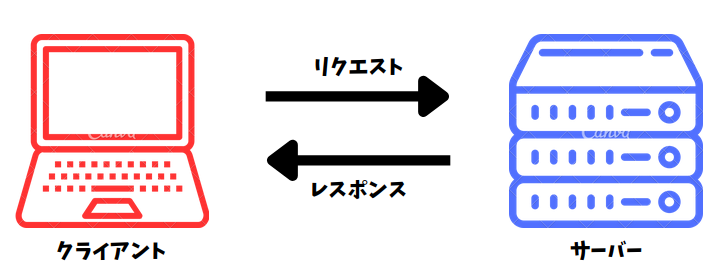
\includegraphics[scale=0.4]{server-and-client.png}
    \end{figure}
\end{frame}

\begin{frame}{WebアプリケーションとWebサイトの違い}
    \begin{itemize}
        \setlength{\parskip}{1.5em}
        \item \textbf{Webサイト}:常に同じHTMLをクライアントに返す.
        \item \textbf{Webアプリケーション}:\\表示内容をクライアントごとに動的に変化するHTMLを返す.
        \begin{enumerate}
            \setlength{\parskip}{1em}
            \item WebブラウザからURLを入力してEnter.\\リクエスト情報がWebアプリに送信(リクエスト).
            \item リクエストがWebアプリに届くと,リソース(HTML, CSS)をデータベースと連携して取得.
            \item ブラウザに返す(レスポンス).
        \end{enumerate}
    \end{itemize}
\end{frame}

\begin{frame}{データベース}
    \begin{itemize}
        \setlength{\parskip}{1.5em}
        
        \begin{columns}
        \begin{column}{0.55\textwidth}
        \item \textbf{データベース}:\\            
        \begin{itemize}
            \setlength{\parskip}{1em}
            \item 構造化した情報,データの組織的な集合\cite{database}.
            \item 通常はコンピュータ・システムに電子的に格納.
            \item \textbf{データベース管理システム(DBMS)}で制御.
        \end{itemize}
        \end{column}            
        \begin{column}{0.3\textwidth}
            \begin{figure}
                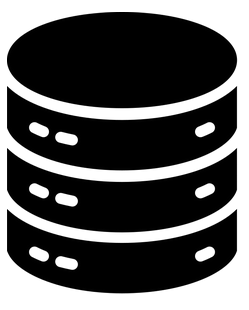
\includegraphics[scale=0.2]{database.png}
            \end{figure}
        \end{column}
        \end{columns}
        \item \textbf{データベース管理システム(Database Management System)}:\\
        \begin{itemize}
            \setlength{\parskip}{1em}
            \item データベースとそのエンドユーザー・プログラムの間でインタフェースとして機能.
            \item データベースの監視・制御を容易にする.
            \item 例)MySQL
        \end{itemize}
    \end{itemize}
    {\tiny \cite{database}データベースとは\url{www.oracle.com/jp/database/what-is-database/}}  
\end{frame}

\begin{frame}{Webアプリケーションの流れ}
    \begin{figure}
        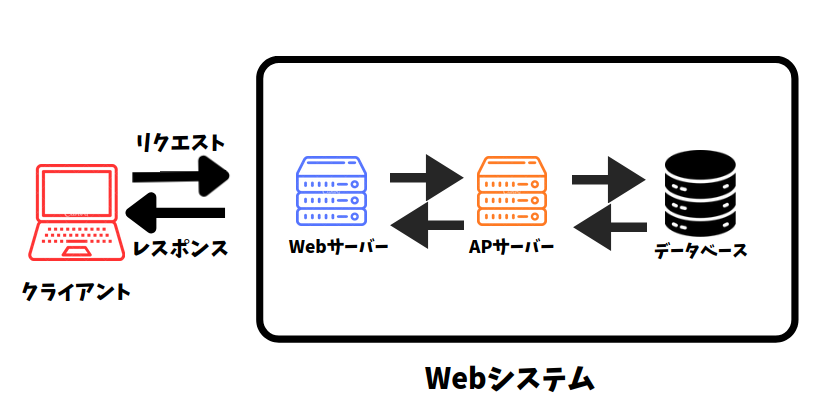
\includegraphics[scale=0.4]{websystem.png}
    \end{figure}
\end{frame}

\begin{frame}{WebサーバーとAPサーバー}
    \begin{itemize}
        \setlength{\parskip}{1.5em}
        \item \textbf{Webサーバー}:\\
        \begin{itemize}
            \setlength{\parskip}{1em}
            \item HTTPリクエストを受け取る\cite{webserver}.
            \item HTMLやCSS,画像などでレスポンスを返す.
        \end{itemize}
        \item \textbf{APサーバー(Webアプリケーションサーバー)}:\\
        \begin{itemize}
            \setlength{\parskip}{1em}
            \item Webサーバから受け取った情報を処理\cite{apserver}.
            \item 必要に応じてデータベースサーバにアクセス.
            \item 動的コンテンツの生成・管理.
        \end{itemize}
    \end{itemize}
    \textbf{Webサーバはユーザーとの窓口.\\APサーバはユーザーのリクエストに応じた対応をおこなうバックヤード.}
\end{frame}

\begin{frame}[allowframebreaks]{Webサイトがブラウザに表示されるまでの大まかな流れ}
    \begin{enumerate}
        \setlength{\parskip}{1em}
        \item Webサーバーにアクセスしてリクエストを送信.
        \item Webサーバーがリクエストを受け取り,解析.
        \item APサーバーが処理を実行.(DB問い合わせなど)
        \item DBから情報を取得.
        \begin{figure}
            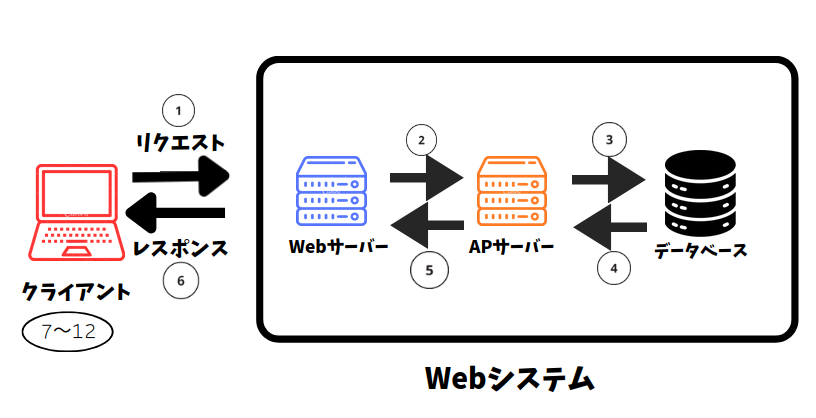
\includegraphics[scale=0.21]{webfloat.png}
        \end{figure}
        \item 静的なHTMLとJavascriptコード or JSONなどのデータをWebサーバーに返す.
        \item Webサーバーがレスポンスとしてクライアントに送信.
        \item ブラウザ(クライアント)がHTMLを解析.DOMツリーを構築.
        \item CSSを読み込み,解析.CSSOMツリーを構築.
        \begin{figure}
            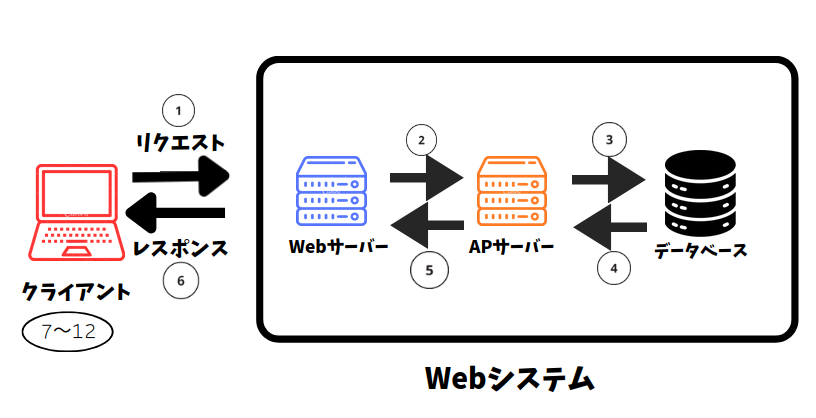
\includegraphics[scale=0.19]{webfloat.png}
        \end{figure}
        \item Javascriptを読み込み実行.動的な処理(データ取得・DOM操作など)を行う.
        \item DOMツリーとCSSOMツリーを合成してレンダーツリーを構築.
        \item レイアウト計算・ペイント.
        \item 画面にレンダリング.
        \begin{figure}
            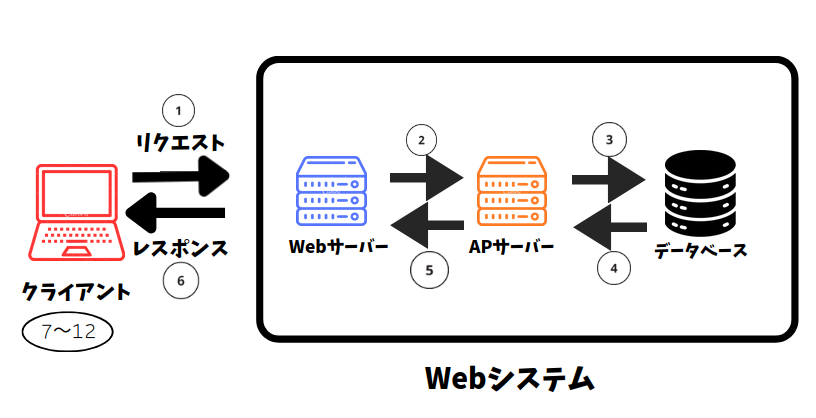
\includegraphics[scale=0.20]{webfloat.png}
        \end{figure}
    \end{enumerate}
    
\end{frame}

\begin{frame}[allowframebreaks]{参考文献}
    \small
    \bibliography{refs}    
\end{frame}
\end{document}
